\subsubsection{Skift-test funktion}
\label{Skift funktion}

Når vi kører mapping runden, checker vi ved hvert Hall-interrupt, om vinkelhastigheden fra gyroen antyder, at der er sket et skift mellem de forskellige banetyper. Undtagelsen er, hvis der er sket et skift mellem store og små sving, da usikkerheden på gyroen er relativt stor, at det kan ske at den kan se et stort sving som et lille, eller omvendt. Derfor antager koden at alle sving der har haft blot én gyro-værdi der antyder et lille sving, er et lille sving, da det er bedre at antage at et stort sving er et lille sving end omvendt. 
\\
Hvis der er sket et skift i vinkelhastigheden, betyder det at vi har skiftet banetype. Derfor gemmes længden og typen af det gamle banestykke i RAM'ene, og vi begynder at tælle det nye banestykke op. Da dette ikke vil ske når vi krydser målstregen, sker dette også når Lap-interruptet siger at mapping runden er slut.
\\
For visuel repræsentation, se figur \ref{fig:Skift Flowchart}

\afterpage{
\begin{figure}
\centering
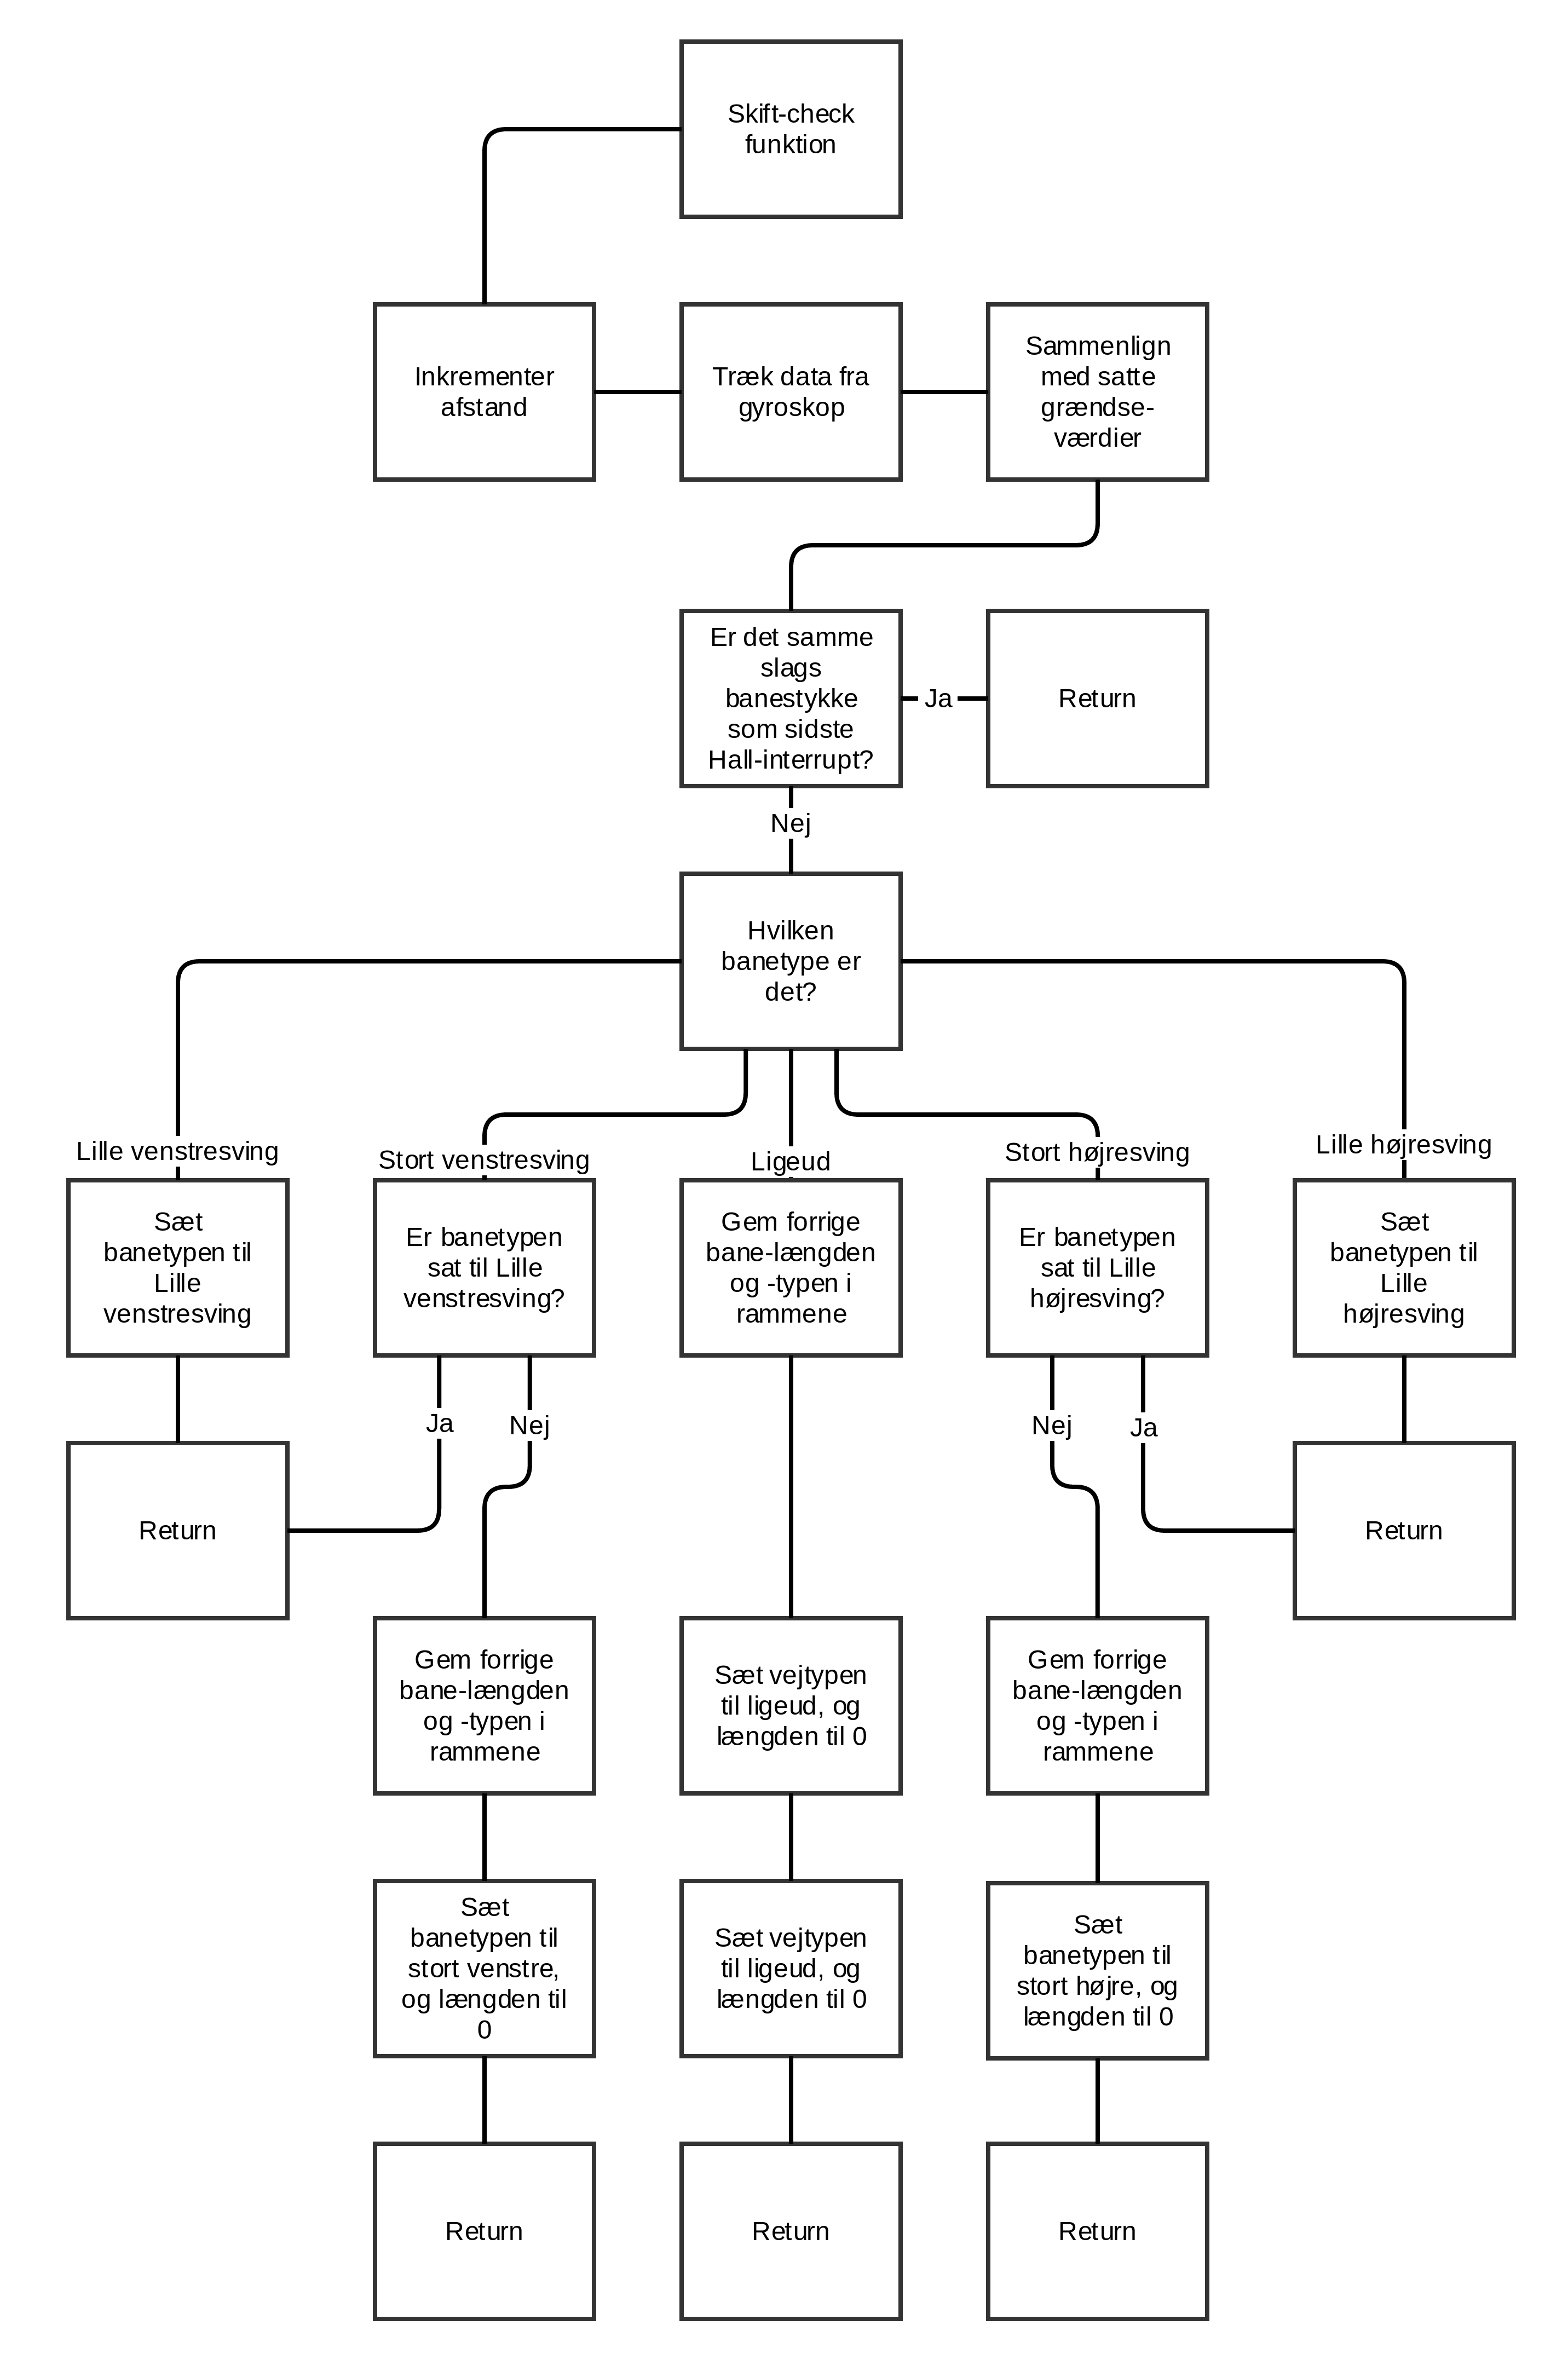
\includegraphics[scale=0.12]{Billeder/skift_check.png}
\caption{Flowchart over Skift-test funktionen.}
\label{fig:Skift Flowchart}
\end{figure}
\clearpage}